
\chapter{Appendix B}\label{appendixb}
This appendix describes the method we used to calculate the time difference and separation between FU3 and FU4 at 06:12 UT on February 2nd, 2015. We used the following method to calculate the clock difference, $\delta t_{c}$  and separation, $d$ between FU3 and FU4 at 06:12 UT on February 2nd, 2015.

The relative clock difference was calculated with a cross-correlation time lag analysis on uniquely-identified trains of microbursts that hit both spacecraft simultaneously. Four time periods with coincident microbursts were hand-picked on February 2nd, 2015 and are shown in Figs. \ref{figure_S1}-\ref{figure_S4}, panels (a) and (b). The cross-correlation time lag analysis was applied to the HiRes time series in panels (a) and (b), and the resulting normalized cross-correlation coefficient as a function of time is shown in panel (c). To validate the peak lag identified in panel (c), FU3's time series was shifted by that lag and is shown in panel (d).

The clock differences from the simultaneous microbursts in Figs. \ref{figure_S1}-\ref{figure_S4} were linearly fit to account for the relative clock drift (${\approx} 20$ ms/hour at this time), giving a value of $\delta t_{c} = 2.28 \pm 0.12 \ s$ at the time of the microburst analyzed here. This time shift was applied to the HiRes data in Fig. 1. A clock difference of $\delta t_{c}  = 2.45^{+ 0.51}_{-0.98}$ s was independently calculated with the FIREBIRD-II telemetry beacon time stamps that were downlinked during operational passes.

We calculate the spacecraft separation, by applying same the cross-correlation time lag analysis on structures assumed to be spatial and are shown in Figs. \ref{figure_S5} and \ref{figure_S6}. The lag from the peak cross-correlation between these events is a sum of the clock difference and time lag due to the spacecraft separation. We interpret the time lag due to the spacecraft separation as the time difference between when the leading satellite observed a stationary spatial feature, to when the trailing satellite observed the same stationary spatial feature. With the method described above, we find the spatial time lag to be $\delta t_{d} = 2.64 \pm 0.12$ s (after we account for the clock difference and its uncertainty). To convert from a spatial time lag to a spacecraft separation, we calculate the satellite velocity. We calculate the velocity using a Two Line Element (TLE), a data format containing the orbit parameters that are used for orbit propagation. With the TLE derived spacecraft velocity, $v = 7.57 \ km/s$, the spacecraft separation was $d = 19.9 \pm 0.9 \ km $.

An independent method to calculate the spacecraft separation was developed. The separation was calculated using TLEs. The TLE from February 2nd was anomalous and was not used in this analysis. Instead, seven TLEs released up to five days after the microburst event were backpropagated, using the SGP-4 algorithm \citep{sgp4} that calculates orbital state vectors with perturbations such as Earth's atmosphere, as well as gravitational effects from the moon and sun. Then the predicted spacecraft separations at the time of the microburst event were averaged to derive a separation of $d = 18.4 \pm 1.5$ km. These two methods give similar separations, which implies that the stationary event assumption used in the cross-correlation time lag analysis is reasonable.

\clearpage

\begin{figure}
%\setfigurenum{S1} %%Change number for each figure
\noindent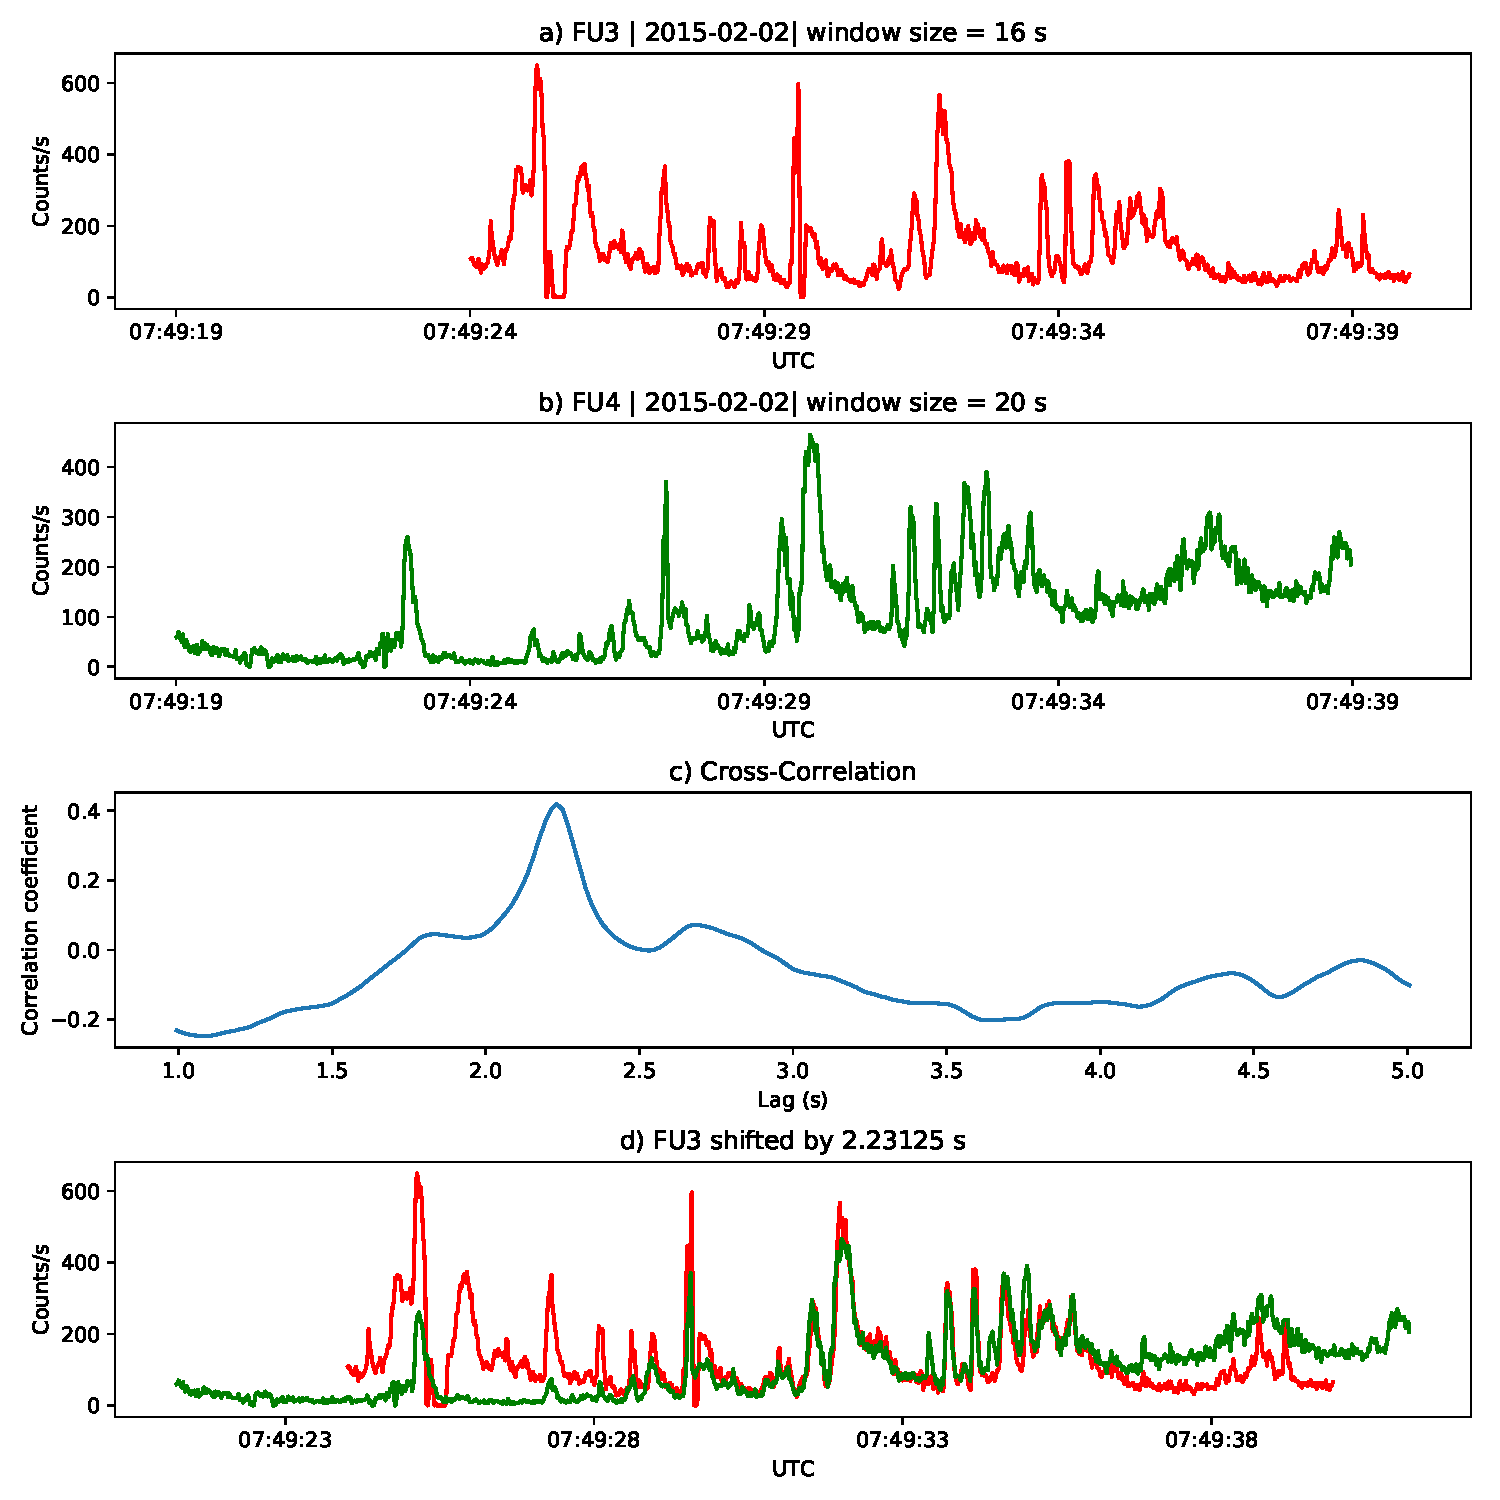
\includegraphics[width=0.8\textwidth]{3_2015-02-02_074931_microburst_crosscorr.pdf}
\caption{Cross-correlation time lag analysis applied to a train of microbursts. Panel (a) and (b) show the count rate from the lowest energy channel. Panel (c) shows the cross-correlation coefficient as a function of time lag. Panel (d) shows the shifted timeseries. Clock difference was 2.23 s.}
\label{figure_S1}
\end{figure}

\begin{figure}
%\setfigurenum{S2} %%Change number for each figure
\noindent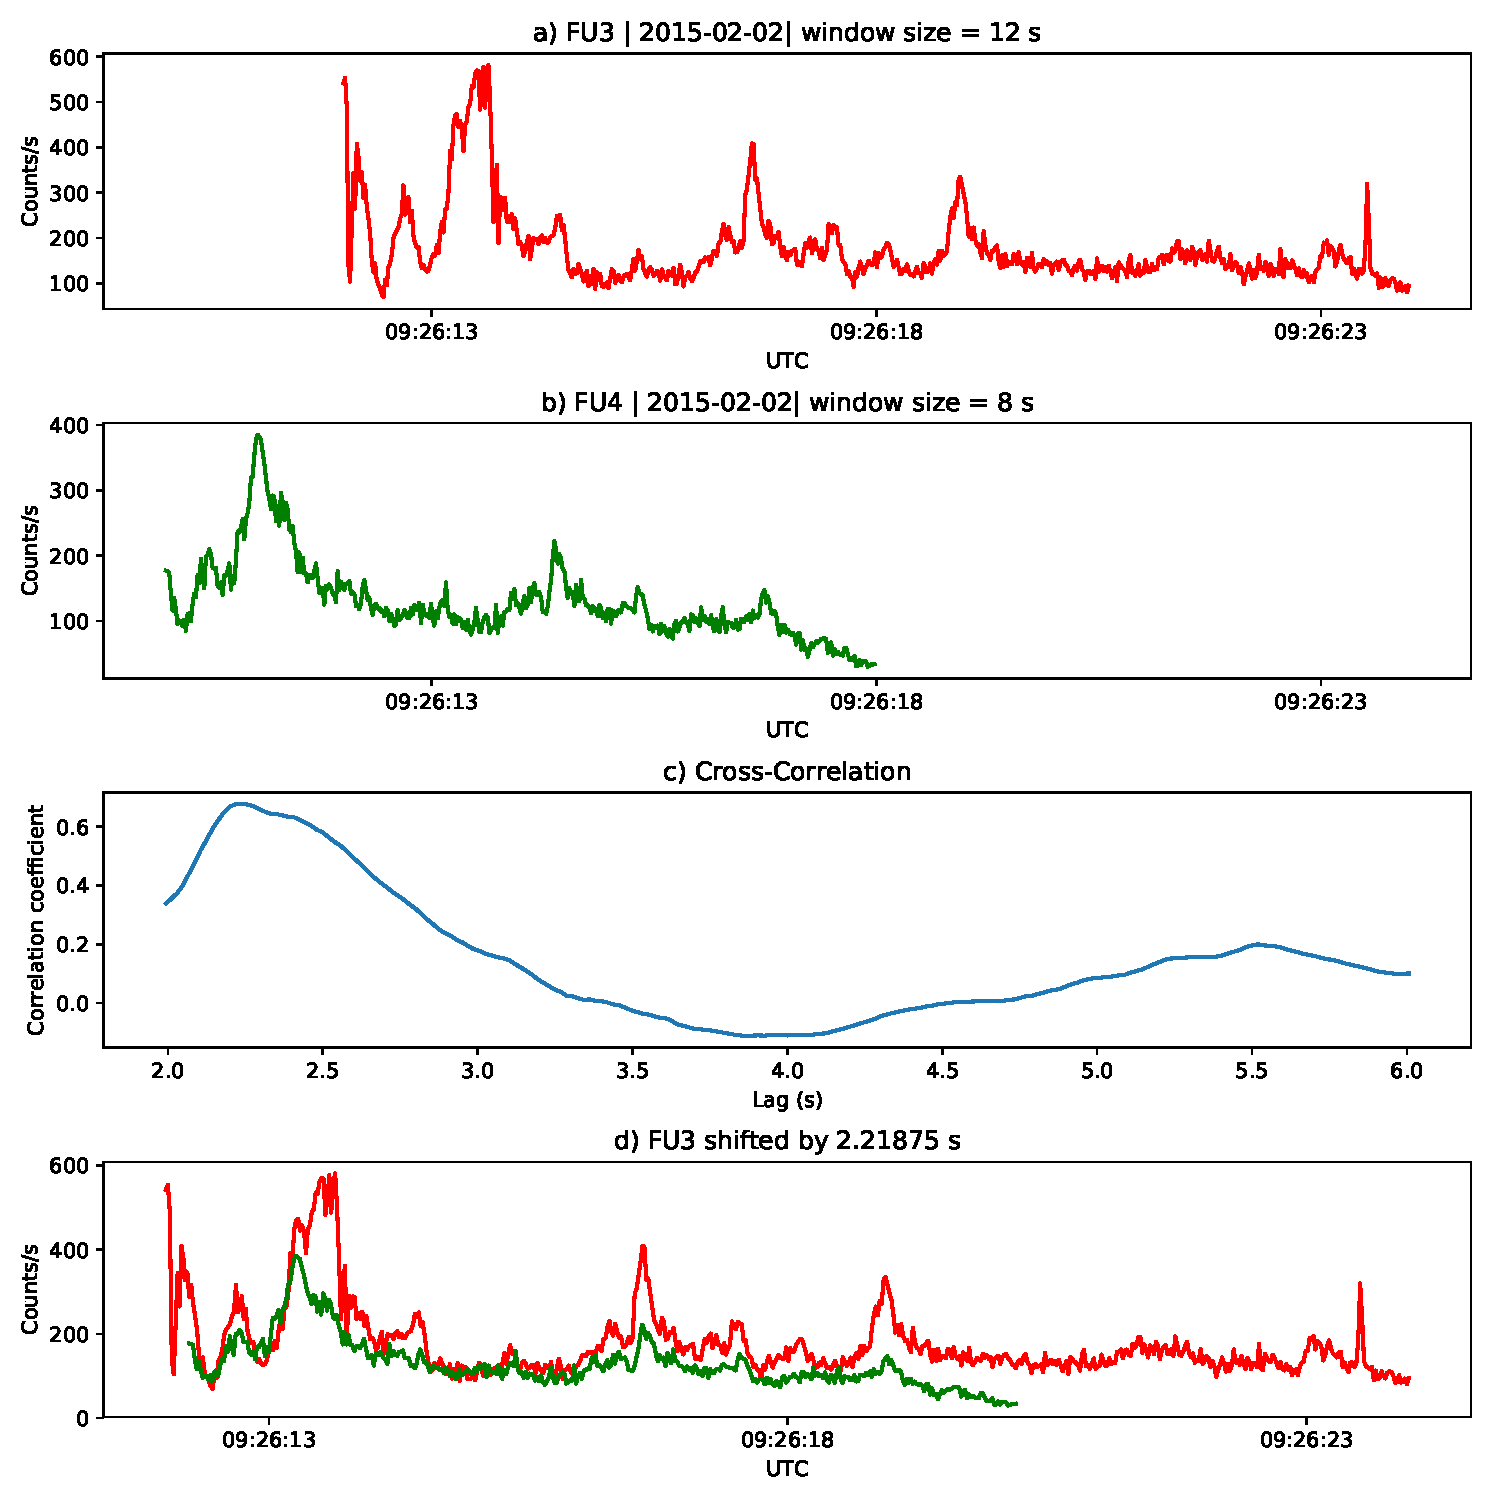
\includegraphics[width=0.8\textwidth]{3_2015-02-02_092613_microburst_crosscorr.pdf}
\caption{Same analysis as Fig. \ref{figure_S1} on a different time period. Clock difference was 2.21 s.}
\label{figure_S2}
\end{figure}

\begin{figure}
%\setfigurenum{S3} %%Change number for each figure
\noindent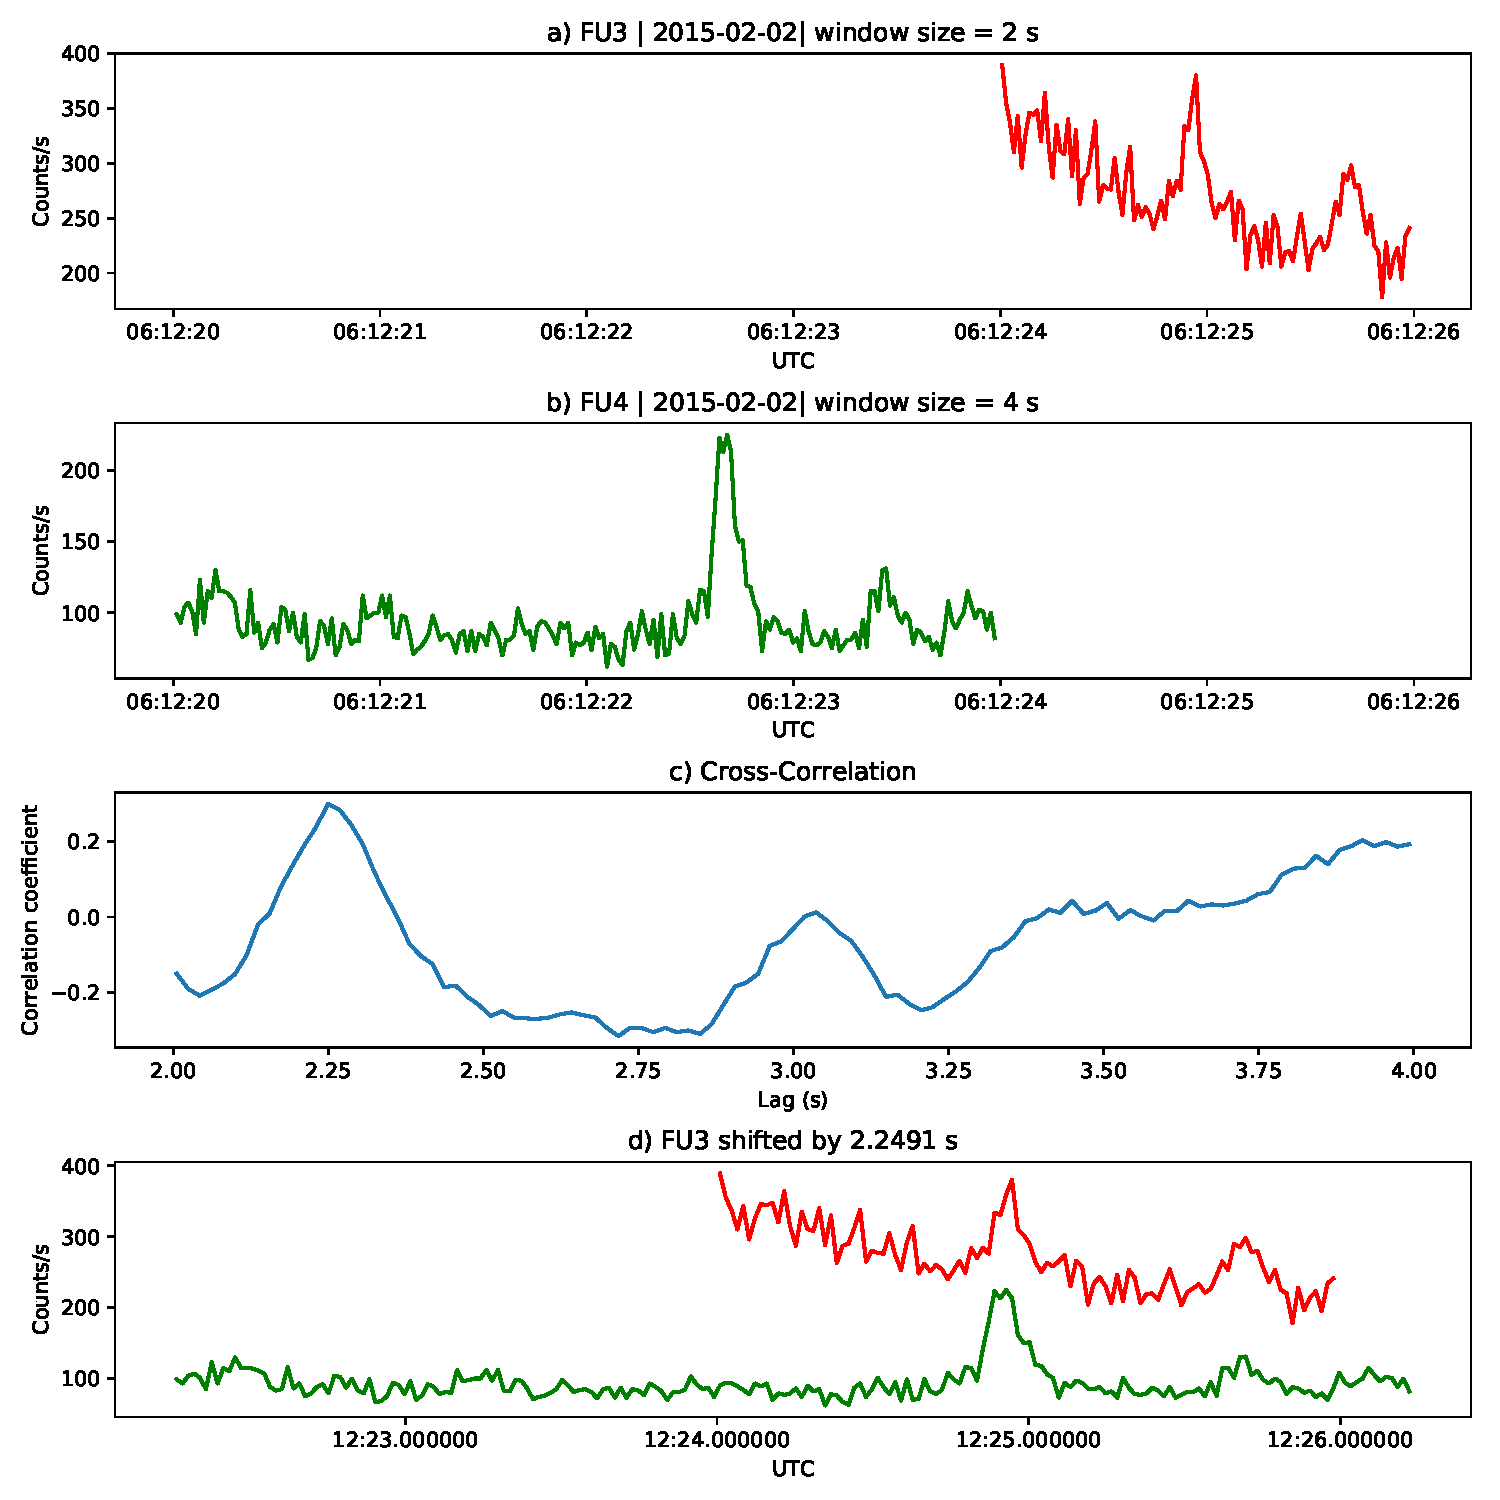
\includegraphics[width=0.8\textwidth]{3_2015-02-02_122300_microburst_crosscorr.pdf}
\caption{Same analysis as Fig. \ref{figure_S1} on a different time period. Clock difference was 2.25 s.}
\label{figure_S3}
\end{figure}

\begin{figure}
%\setfigurenum{S4} %%Change number for each figure
\noindent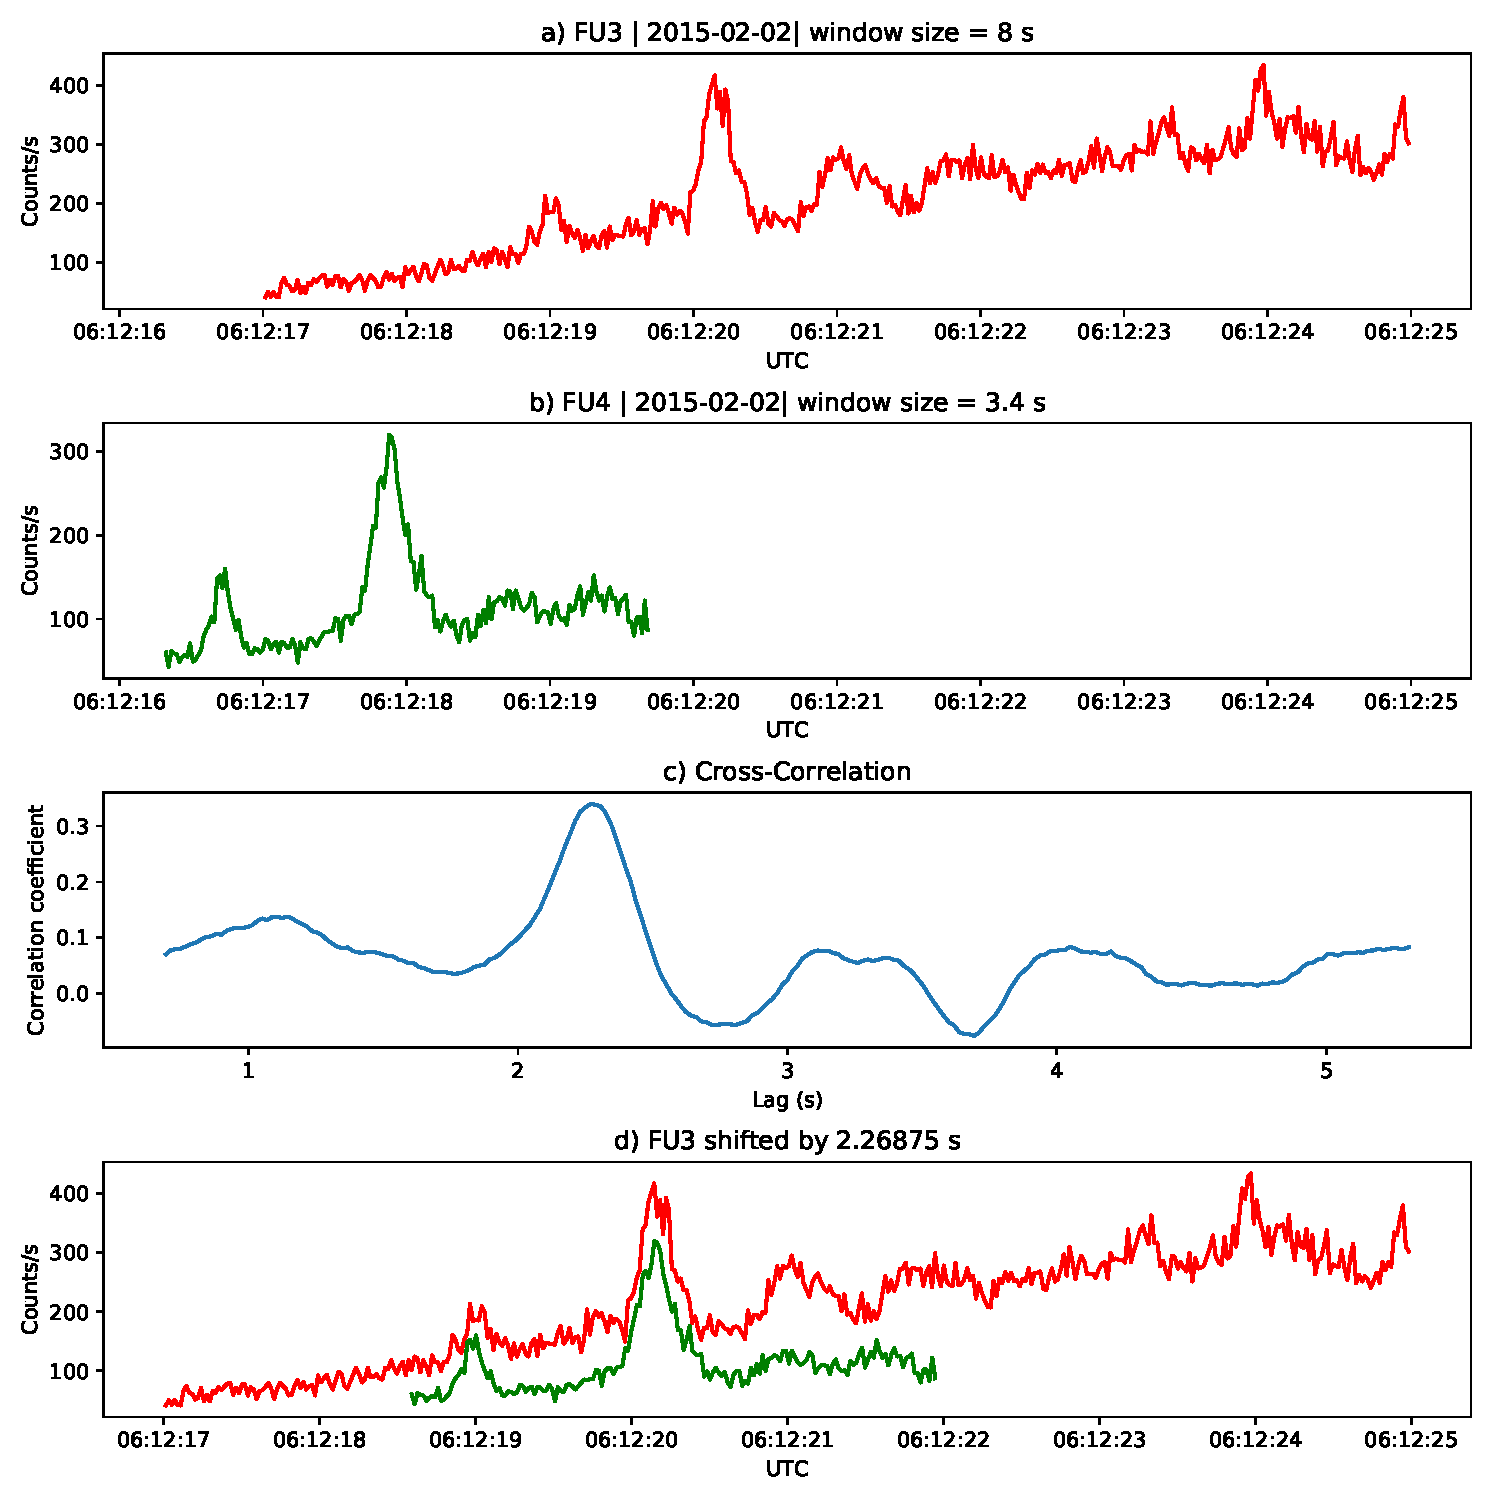
\includegraphics[width=0.8\textwidth]{3_2015-02-02_061217_microburst_crosscorr.pdf}
\caption{Same analysis as Fig. \ref{figure_S1} on a different time period. Clock difference was 2.27 s.}
\label{figure_S4}
\end{figure}

\begin{figure}
%\setfigurenum{S5} %%Change number for each figure
\noindent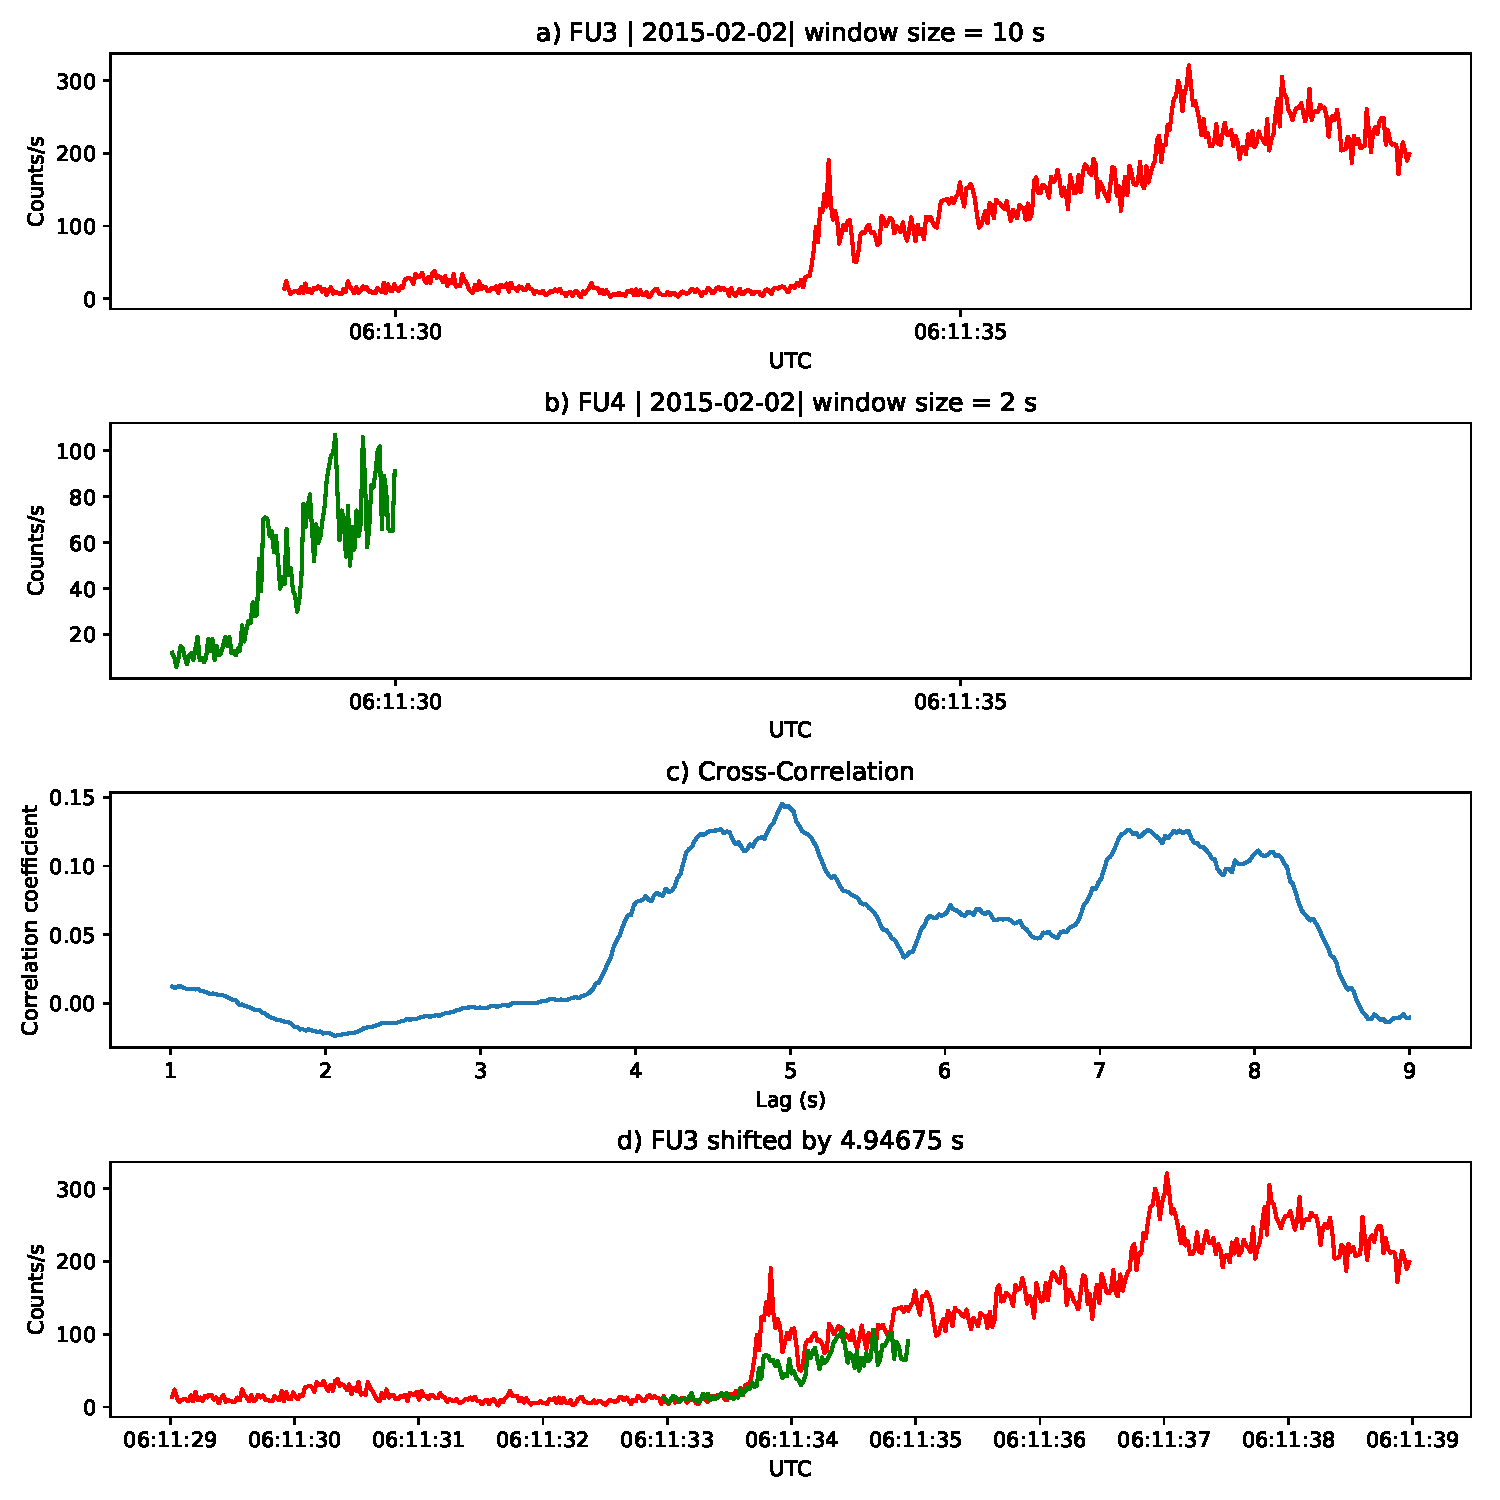
\includegraphics[width=0.8\textwidth]{3_2015-02-02_061129_stationary_crosscorr.pdf}
\caption{Same cross-correlation time lag analysis applied to stationary spatial structures. The cross-correlation lag between these events is a sum of the clock difference and time lag due to the spacecraft separation. The lag derived at this time was 4.95 s.}
\label{figure_S5}
\end{figure}

\begin{figure}
%\setfigurenum{S6} %%Change number for each figure
\noindent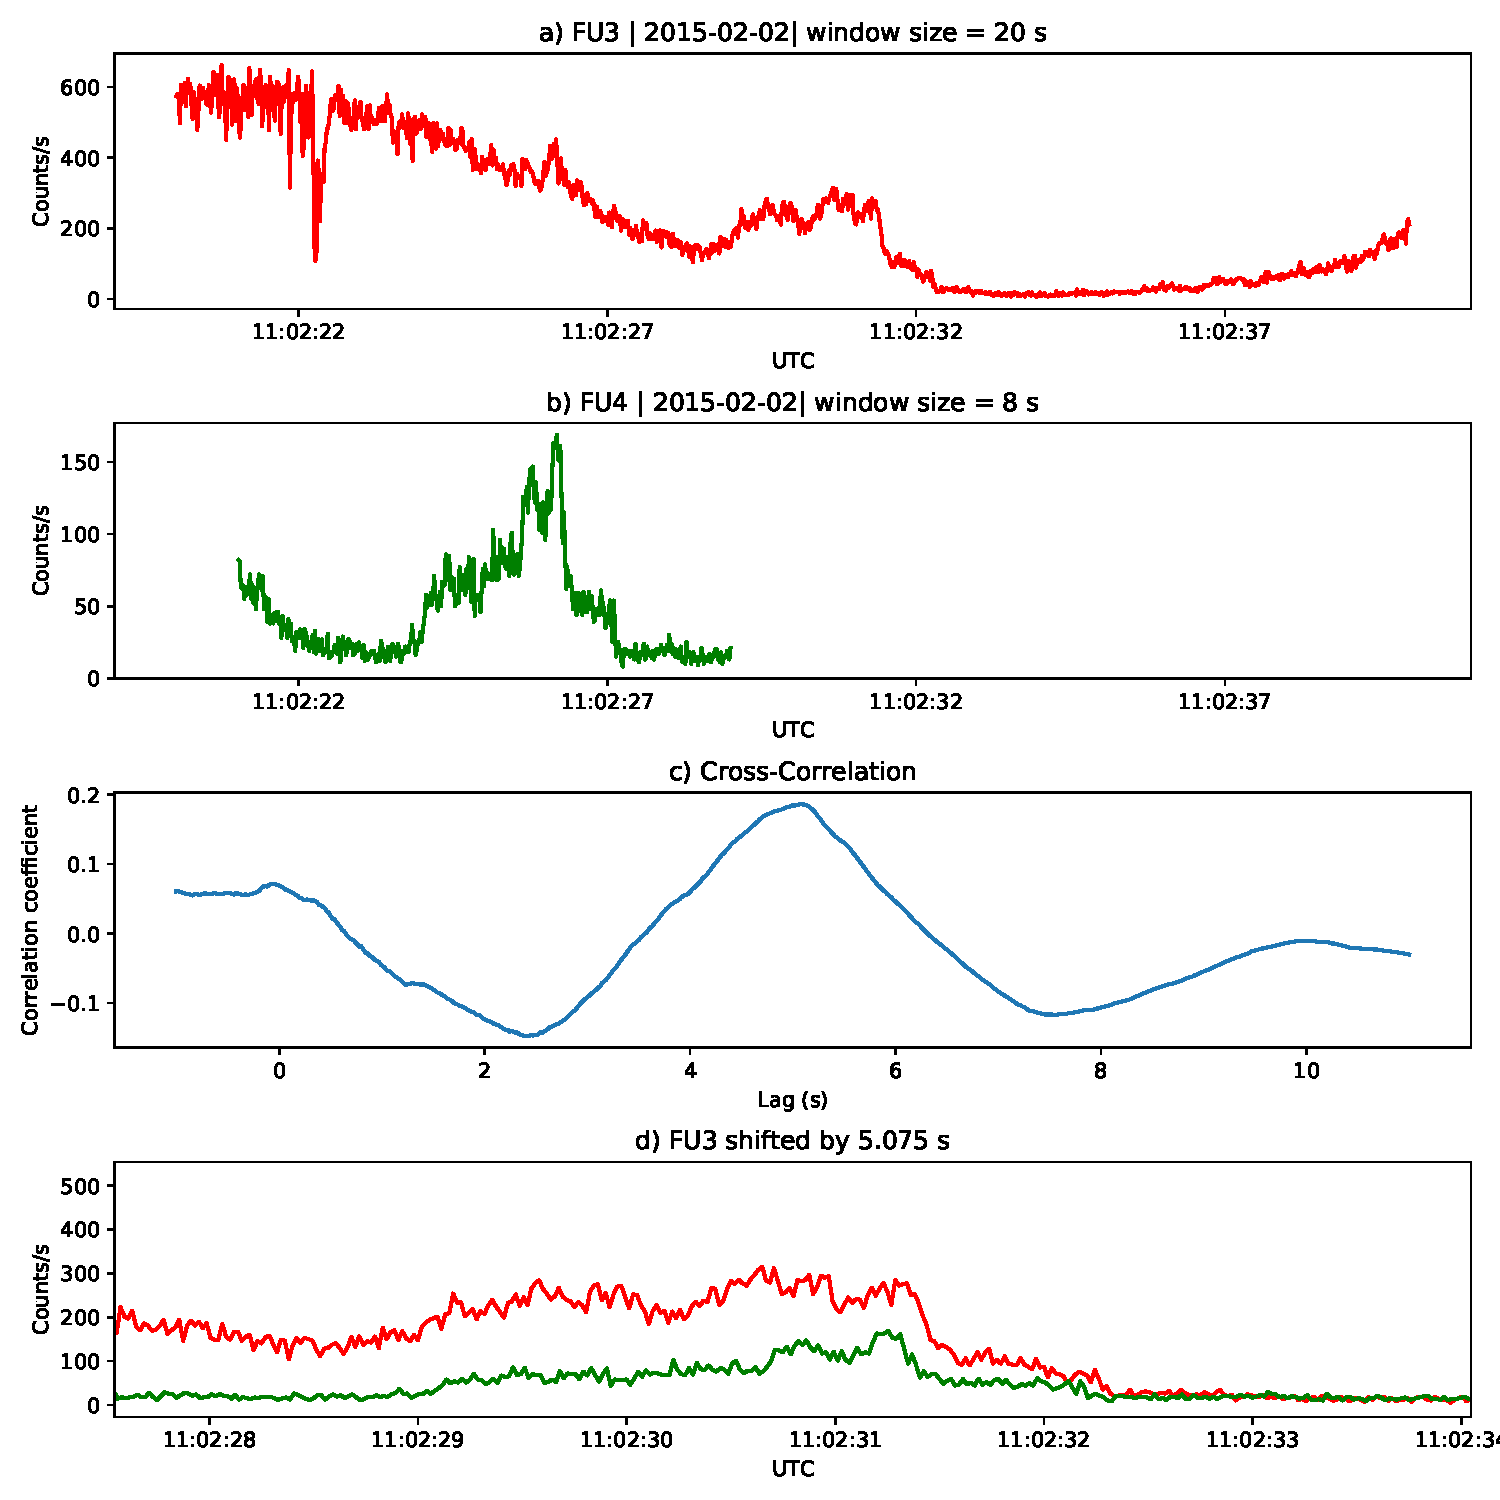
\includegraphics[width=0.8\textwidth]{3_2015-02-02_110228_stationary_crosscorr.pdf}
\caption{Same analysis as Fig. \ref{figure_S5} applied to a different stationary spatial feature. The lag derived at this time was 5.01 s.}
\label{figure_S6}
\end{figure}
